% 翻折 例3：正方形边1，△ABF 沿 AF 翻折，B->B' 落在 AC 上，BF=tan22.5°=√2-1
\documentclass[tikz,border=4pt]{standalone}
\usepackage{ctex}
\usepackage{amsmath}
\usetikzlibrary{calc}
\begin{document}
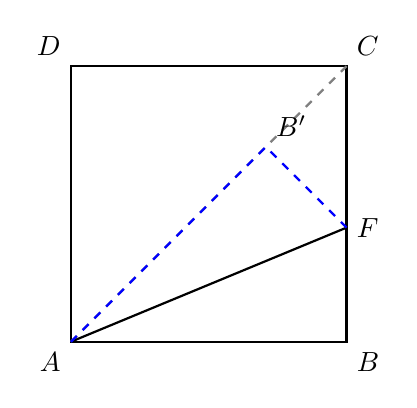
\begin{tikzpicture}[scale=3.5, thick]
  % 正方形 A=(0,0) B=(1,0) C=(1,1) D=(0,1)
  \coordinate (A) at (0,0);
  \coordinate (B) at (1,0);
  \coordinate (C) at (1,1);
  \coordinate (D) at (0,1);
  % F 在 BC 上 BF = √2-1 ≈ 0.4142
  \coordinate (F) at (1, 0.4142);
  % B' 在对角线 AC 上, AB'=1 -> B' = (√2/2, √2/2) ≈ (0.7071, 0.7071)
  \coordinate (Bp) at (0.7071, 0.7071);
  \draw (A)--(B)--(C)--(D)--cycle;
  \draw[gray, dashed] (A)--(C);
  \draw (A)--(F);
  \draw (B)--(F);
  \draw[blue, dashed] (A)--(Bp)--(F);
  \node[below left] at (A) {$A$};
  \node[below right] at (B) {$B$};
  \node[above right] at (C) {$C$};
  \node[above left] at (D) {$D$};
  \node[right] at (F) {$F$};
  \node[above right] at (Bp) {$B'$};
\end{tikzpicture}
\end{document}
